 
\section{共点力平衡和力矩平衡} 
\subsection{共点力平衡}
虽然名字里带个平衡,但不代表本章的研究对象全部都受力平衡!本节旨在细致研究物体的受力情况,以便后续的学习.
\subsubsection{力的正交分解}
力$\boldsymbol{\mathrm{F}}$是一个矢量.这意味着它有方向!因此类似运动,我们可以将一个力分解在两个相互垂直的方向上.如图2-1所示.我们不妨设其中一个方向为x轴,另一方向为y轴,$\boldsymbol{\mathrm{F}}$与x轴的夹角为$\theta$,那么$F_x=F\cos\theta,F_y=F\sin\theta$,如图\ref{Fzjfj}所示.由此,我们将一个力$\boldsymbol{\mathrm{F}}$分解成了两个互相垂直的力.这就是力的正交分解.\begin{figure}[htp]\centering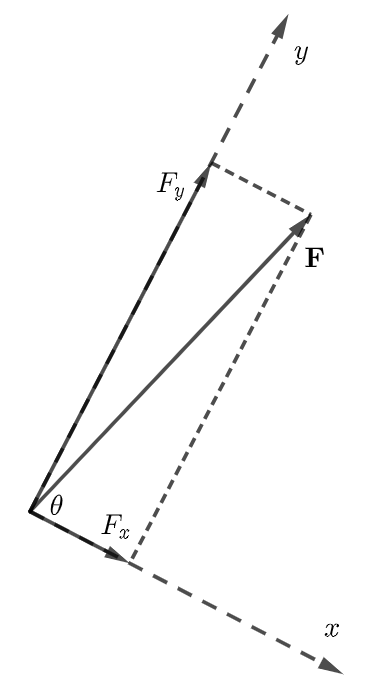
\includegraphics[width=3.5cm]{6-2}\caption[力的正交分解]{力的正交分解示意图}\label{Fzjfj} \end{figure}
\subsubsection{方向上的平衡}
在上一节中我们学会了如何将力$\boldsymbol{\mathrm{F}}$分解到两个方向.而所谓\textbf{平衡}想必大家都早有耳闻:这代表着在任何方向上(或某一特定方向上,如x轴或y轴)所受合理为零,表达式为:\begin{equation}
	\Sigma \boldsymbol{\mathrm{F}}_p=0
\end{equation}


其中$p$表示研究的某一方向.
\subsubsection{二力共线和三力共点}
接着延续上一节的结论:如果一物体所受合力为0,即$\Sigma  \boldsymbol{\mathrm{F}}_x=\Sigma \boldsymbol{\mathrm{F}}_y=0$,那么有: 
\newcounter{DL}[section]    %定义新计数器TH
\renewcommand{\theDL}{\thesection.\arabic{DL}}  %重新定义计数器命令\theTH的显示形式
\newcommand{\theorem}[1][]{\par\textbf{定理}\refstepcounter{DL}\textbf{\theDL}(#1)\quad}  %新定义定理命令
\theorem[平衡力]\label{dl1.1}


(1)如果该物体受两个力,那么它们共线等大;


(2)如果该物体受三个力,那么它们共点.

接下来我们证明\textbf{定理\ref{dl1.1}}.


{\CJKfamily{zhkai} 证明:}


{\CJKfamily{zhkai}\label{dl1.1-1} (1)如果该物体仅受恰好两个力,不妨设它们为$\boldsymbol{\mathrm{F}_1}$和$\boldsymbol{\mathrm{F}_2}$,并将$\boldsymbol{\mathrm{F}_1}$设为正方向,$\boldsymbol{\mathrm{F}_2}$与$\boldsymbol{\mathrm{F}_1}$的夹角为$\theta$.于是在$\boldsymbol{\mathrm{F}_1}$直线方向合力$F_1=\boldsymbol{\mathrm{F}_1}+\boldsymbol{\mathrm{F}_2}\cos\theta=0$,$F_2=\boldsymbol{\mathrm{F}_2}\sin\theta=0$,因此$\sin\theta=0$,所以$\theta=k\pi,k\in \mathbb{N}$.而如果$k\in \left\lbrace \mathbb{N}|k=2n,m\in N \right\rbrace $,此时$\boldsymbol{\mathrm{F}_1}+\boldsymbol{\mathrm{F}_2}=0$,又$\boldsymbol{\mathrm{F}_1},\boldsymbol{\mathrm{F}_2}>0$,矛盾.故$\theta=(2n+1)\pi,n\in\mathbb{N}.$这意味着$\boldsymbol{\mathrm{F}_1}$和$\boldsymbol{\mathrm{F}_2}$共线.且此时$\boldsymbol{\mathrm{F}_1}-\boldsymbol{\mathrm{F}_2}=0,$即$\boldsymbol{\mathrm{F}_1}=\boldsymbol{\mathrm{F}_2}$.}


{\CJKfamily{zhkai}\label{dl1.1-2-1} (2)如果该物体受三个力,还是设它们为$\boldsymbol{\mathrm{F}_1}$,$\boldsymbol{\mathrm{F}_2}$和$\boldsymbol{\mathrm{F}_3}$.仍然认为$\boldsymbol{\mathrm{F}_1}$为正方向,$\boldsymbol{\mathrm{F}_2}$与$\boldsymbol{\mathrm{F}_1}$夹角$\alpha$,$\boldsymbol{\mathrm{F}_3}$与$\boldsymbol{\mathrm{F}_1}$夹角$\beta$.类比\ref{dl1.1-1}的证明(1),有}\\
\[
\left\{  \begin{lgathered}
	\boldsymbol{\mathrm{F}_1}+\cos\alpha\boldsymbol{\mathrm{F}_2}+\cos\beta\boldsymbol{\mathrm{F}_2}=0\\
	\sin\alpha\boldsymbol{\mathrm{F}_2}+\sin\beta\boldsymbol{\mathrm{F}_3}=0
	\end{lgathered} \right.
\]


{\CJKfamily{zhkai} 这个方程其实并非最优证法.有兴趣的读者可以尝试解它.当然,一般来说,你会败兴而归.我们介绍一种更普遍、简单的办法:\\\textcircled{1} 将任意两个力分方向合成,使得$x$方向与$\boldsymbol{\mathrm{F}_1}$在同一直线.\\\textcircled{2}将合成所得的力与$\boldsymbol{\mathrm{F}_1}$再合成,利用\ref{dl1.1-1}的证明(1)的结论即可得到:两个力的合力和另一个力共线,这意味着它们一定共顶点!而两个力的合力一定经过它们的交点(如果有的话),因此这三个力共点.}\\


{\CJKfamily{zhkai} 思考:为什么两个力的合力一定经过它们的交点(如果有的话)?如果有四个力,}\textbf{定理\ref{dl1.1}}{\CJKfamily{zhkai} 还成立吗?需要做什么改动?}
\subsection{力矩平衡}
\subsubsection{力矩五要素和力矩的计算}
让我们回到正题.上一节中,我们讲了平衡力的一些性质.本节讲述力矩.


力矩$M$在初中已经学过,有五要素为支点O,动力(组)$F_1\sim F_n$,动力臂(组)$L_1\sim L_n$,阻力(组)$F_{n+1}\sim F_m$,阻力臂(组)$L_{n+1}\sim L_m$,其中$m>s$.每一个力$F_i$都有其对应的力臂$L_i$和力矩$M_i=F_iL_i$.


那力矩平衡的表达式?相信各位应该也不陌生吧:$\Sigma M_p=\Sigma M_q$.其中$M_p$和$M_q$分别表示动力力矩和阻力力矩.
\subsubsection{变力平衡}
当恒力或非恒力与物体以一夹角做功时,物体会改变运动状态.不同的角度和力都会对该力的力矩造成影响,而如果想不改变物体运动状态和力的方向(大小),我们就需要改变力的大小(方向).如果一个力作用在离支点O$l$的点A,力的方向与AO夹角为$\theta$,那么该力力矩为$M=Fl\sin\theta$,注意与运动学中更为常见的$\cos\theta$做区分.
\subsection{1.2例题}
\subsection{1.2习题}